\RequirePackage[T1]{fontenc}
\documentclass[10pt,conference]{IEEEtran}
\usepackage{amsmath,amssymb,amsthm,graphicx,booktabs,array,url,flushend}
\usepackage[hidelinks]{hyperref}
\usepackage{tikz}
\usetikzlibrary{arrows.meta,positioning}
\emergencystretch=2em
\newtheorem{theorem}{Theorem}
\newtheorem{lemma}{Lemma}
\newtheorem{proposition}{Proposition}
\theoremstyle{definition}
\newtheorem{definition}{Definition}
\newtheorem{remarknum}{Remark}
\newcommand{\code}[1]{\texttt{#1}}
\newcommand{\G}[1]{G#1}
\newcommand{\tool}{ReleaseWeave}
\newcommand{\lang}{RIL}
\begin{document}
\title{Recovering Versioned Releases Across Build and Publish Boundaries}
\maketitle
\begin{abstract}
Mixed releases must coordinate local package outputs with published artifacts:
a Docker base image may include an npm engine, while another image needs that
published base and an npm SDK. Incorrect ordering starts builds too early;
incomplete recovery can forget unfinished packages or change their versions.
We present a saga-inspired release protocol that records each package's
completion in Git and resumes unfinished work through the same release command.
Commit messages control affected packages, holds and prereleases. Shared
configuration supports Windows/Linux workflows; an agent skill guides
commit diagnostics, plan inspection, tests and CI releases.
Planning is a pure function of fixed inputs, allowing cached plans without
changing decisions. Specified extensions distribute tasks and releases across
workers and repositories.
The model explains when dependencies are available and why each consumer must
retain its own pending work. It establishes eight conditional guarantees,
including stable retry versions and idempotent recorded releases.
Exploratory outreach covers at least 211 repositories, without estimating defect
prevalence. All 120 controlled fault episodes recover after repair; an analytical
alternative that discards intent when its provider succeeds loses work in 84.
Real-registry, CI, historical replay and scale experiments provide complementary
evidence, including google-cloud-node.
Native Windows equivalence and distributed execution remain unevaluated;
external effects require safe repetition or reconciliation.
Linux and LLVM results will be presented in the report.
\end{abstract}
\begin{IEEEkeywords}
software release engineering, continuous integration and delivery,
dependency scheduling, recovery, idempotence
\end{IEEEkeywords}
\section{Introduction}
\label{sec:intro}
Consider two npm workspace packages: a shared asset library and a UI package
that imports it, followed by two Docker images. The dependent UI package
consumes its provider's local build output, and the first image packages the
built UI. The second image uses the first as its base; when built by an isolated
registry-based builder, it must pull the new base version from a registry.
Building all packages before publishing any of them is not a valid schedule
for this release. Serializing every package through both stages is sufficient
but also forces local-artifact consumers to wait for uploads they do not need.

Interruption makes the problem harder. If both npm packages and the base image have
published but the final image fails, a repeated command should finish the
remaining release. It should neither forget that image because its providers
have already released nor assign a different version solely because the first
attempt made progress. A release engine must therefore answer three questions:
which versions are owed, which stages may run, and which obligations remain
after a failure. These questions interact, but require different state.

Release engineering spans more than compilation~\cite{adams}. A heterogeneous
release writes to independently administered package registries, container
registries, and deployment services. They provide no shared atomic commit.
The resulting execution resembles a saga~\cite{sagas}: individual steps commit
separately, and recovery must account for the work that already succeeded.
For published artifacts, deletion may be unavailable or operationally
unacceptable. Our protocol therefore uses forward recovery. It completes or
reconciles outstanding work rather than assuming that every external effect
has a compensating action.

Workflow engines can express a build/publish DAG. Existing release tools also
compute versions and coordinate publication~\cite{lerna,nx,changesets,
releaseplease,semanticrelease}. The question studied here is how to compose
stage ordering with a release ledger so that successful providers do not
erase their failed consumers' obligations. The key rule is consumer-based
admission: a propagated unit of intent remains pending according to the
consumer's own release window, even when the originating package has already
recorded its release. A second distinction separates intent accumulated over
a prerelease train from fresh work not yet delivered.

We present \tool{}, an implementation of this protocol, and \lang{}, its
release-intent language. These names are pseudonyms for anonymous review;
reported version numbers identify the evaluated artifacts. The implementation
uses Git history and tags as its release ledger and ordinary commands for
build and publish stages. It requires no additional persistent release-state
database. That claim concerns orchestration state, not the storage used by
registries, build tools, or deployed applications.

A package is a versioned release unit: software, specifications, and
documentation use the same intent, dependency, command, and completion
interfaces. The protocol accommodates different build tools and registries;
its guarantees require conforming integrations, not a particular language.
The same graph also gives provisioned CI a stable entry point for affected
tests and releases as packages evolve; configuration still records each new
package, and new credentials or runners can require workflow changes.

The paper makes three contributions:
\begin{itemize}
\item An ecosystem-independent, saga-inspired release protocol combining
local-artifact and published-artifact dependencies with explicit release
intent and per-package completion records
(Section~\ref{sec:system}).
\item A self-contained model with deterministic planning and eight recovery,
discharge, and scope/channel guarantees under stated assumptions
(Sections~\ref{sec:model}--\ref{sec:guarantees}). Counterexamples explain why
consumer windows and stable retry predicates matter.
\item An evaluation of a released binary using differential planning,
targeted vectors, injected failures, historical replay, and scale measurements
(Section~\ref{sec:eval}), with the model-to-implementation gap made explicit.
\end{itemize}

The mathematical contribution is the admission and discharge discipline,
not a new topological-sorting or Git-storage primitive.

\section{System and Release Protocol}
\label{sec:system}
\label{sec:impl}
\subsection{A Release Crossing Two Availability Boundaries}
\label{sec:motivation}
Our running example has three packages: \code{assets} produces an npm build,
\code{base} packages that output into a Docker image, and \code{app} builds
from the versioned \code{base} image. Arrows in Fig.~\ref{fig:stages} run from
provider to consumer. The second builder obtains its base through a registry;
we do not assume that it shares the first builder's local image store.

\begin{figure*}[t]
\centering
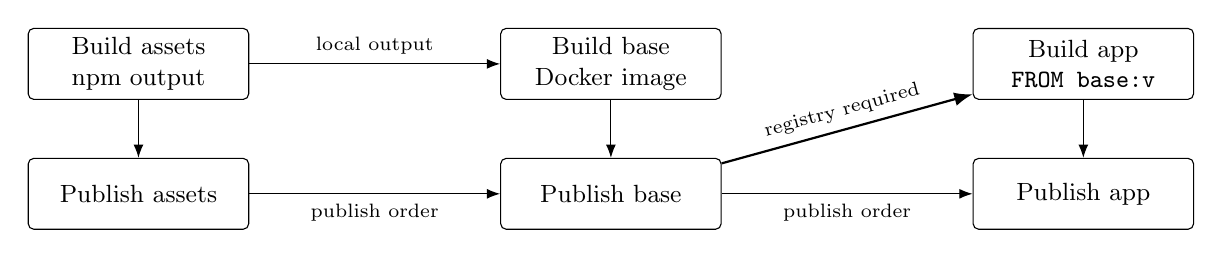
\begin{tikzpicture}[>=Latex,node distance=16mm,
 every node/.style={font=\small},
 stage/.style={draw,rounded corners=2pt,minimum width=28mm,minimum height=9mm,align=center}]
\node[stage] (ab) at (0,0) {Build assets\\npm output};
\node[stage] (bb) at (6,0) {Build base\\Docker image};
\node[stage] (cb) at (12,0) {Build app\\\texttt{FROM base:v}};
\node[stage] (ap) at (0,-1.65) {Publish assets};
\node[stage] (bp) at (6,-1.65) {Publish base};
\node[stage] (cp) at (12,-1.65) {Publish app};
\draw[->] (ab) -- node[above,font=\scriptsize]{local output} (bb);
\draw[->] (ab) -- (ap);
\draw[->] (bb) -- (bp);
\draw[->,thick] (bp) -- node[above,sloped,font=\scriptsize]{registry required} (cb);
\draw[->] (cb) -- (cp);
\draw[->] (ap) -- node[below,font=\scriptsize]{publish order} (bp);
\draw[->] (bp) -- node[below,font=\scriptsize]{publish order} (cp);
\end{tikzpicture}
\caption{Stage dependencies, not a measured timeline. Publishing \code{assets}
may overlap building \code{base}. Building \code{app} must wait for
\code{base}'s publication. Availability modes are configured requirements:
an npm dependency fetched from a registry would also require publication.}
\label{fig:stages}
\end{figure*}

An npm label alone does not justify overlap: \code{base} must actually consume
local output. Similarly, Docker does not universally require a push between
builds; the registry barrier is needed for the isolated-builder consumption
mode in this example. The provider setting
\code{isBuildWaitingPublish: true} declares that its consumers require its
published artifact. Here it is set on \code{base}, while \code{assets} uses
the default local-build mode. Consumer publication is ordered after provider
publication in both modes. A missing stage script is a no-op stage, not a
reason to omit dependencies or completion records.

Suppose \code{assets} is at version 1.4.2, \code{base} at 0.8.2, and
\code{app} at 2.1.0. An intent to release an assets feature and patch all
transitive consumers plans versions 1.5.0, 0.8.3, and 2.1.1. After the first
two packages publish and are recorded, \code{app} fails. A planner that only
propagates from \emph{currently unreleased providers} can now lose
\code{app}: the original provider is no longer pending, so its intent reaches
nobody. The package is an orphan in the release ledger. Our planner instead
asks whether \code{app} has received that intent. Its own pending window is
unchanged, so a retry still owes version 2.1.1.

\subsection{From Repository Inputs to a Plan}
\label{sec:ccme}
The planner reads a fixed repository revision, package definitions, dependency
edges, commit messages, and release tags. Configuration supplies build and
publish commands and availability requirements; manifests can supply package
and dependency identities. The plan specifies selected packages, next
versions, and reasons before any external publication occurs. Changed
inputs require a new plan; a preview is not an authorization for arbitrary
later repository states.

Release intent extends Conventional Commits~\cite{cc}. For example,
\code{feat(assets)\^{}\^{}: add theme assets} directly requests a minor
release of \code{assets} and propagates patch intent to transitive consumers.
An unmarked unit affects its own scope only. A scope can explicitly name
packages or be derived from changed paths. A commit can contain multiple
independent units, each retaining its own source set and propagation depth.
The formal model consumes normalized units, not a particular parser syntax.
The complete language grammar is outside this paper~\cite{ccme2}.

Version bumps and prerelease channels are separate axes. A unit can request a
channel transition without requesting a bump, and channel resolution can
restrict which propagated bumps are meaningful. Cancellation and correction
operate on pending intent; they do not unpublish existing artifacts. An exact
version directive pins a release, while a hold retains work without admitting
the package to the current plan. These controls explain the predicates needed
by the model; their CLI forms are not additional scientific contributions.

\subsection{Execution, Recording, and Recovery}
For each selected package, the executor schedules version reconciliation,
build, and publish work. A consumer's version/build work waits for provider
builds, or for provider publications when their availability mode requires it.
Build and publish tasks have separate concurrency limits. Independent ready
tasks may proceed concurrently; deterministic planning does not require a
fixed temporal order for independent completion events.

Successful publication creates a per-package completion obligation. The model
records it immediately as a tag. The implementation also has configured
recording and finalization steps, whose failures must be reported; their
crash boundaries are not assumed atomic with an arbitrary publish command.
The next invocation reconstructs outstanding work from the resulting records.
This avoids a separate persistent recovery database, but depends on preserving
and making the release tags available. A lock prevents cooperating release
jobs from writing the same remote release concurrently. It does not make
registry operations transactional or prevent an administrator from rewriting
history outside the protocol.

Two failure cases must remain distinct. If a publish is known to have failed,
its obligation stays pending. If the external operation succeeds but its
response or completion record is lost, an absent tag cannot distinguish that
success from failure. The integration must reconcile the artifact's identity
or use a publisher that safely accepts repetition before recording completion.
Forward recovery does not by itself solve this uncertainty~\cite{helland12}.
The mathematical claims below refer to the recorded state and make their
retry assumptions explicit.

\subsection{Applicability and Practical Limits}
The graph may contain one package: the same record-and-retry discipline still
applies even though there is no propagation. A monorepo supplies several
packages under one history. In a polyrepo, a control repository records
submodule pointers and the release graph; its commits and tags provide the
single history and ledger used by the model. The linked repositories keep
their own histories. This is a construction over a control history, not an
atomic transaction across independent Git repositories.

The integration contract has four parts: stable package and version
identities; declared dependencies and availability requirements; commands
whose successful exit means their promised stage has completed; and durable,
trustworthy completion records. Repeated publication must either be safe or
reconciled when its outcome is uncertain. These requirements also admit a
specification released as versioned files: validation or rendering can be its
build stage, and publishing the bundle its publish stage. This is a common
protocol for conforming integrations, not an assertion that every existing
release workflow or version scheme fits the model. In particular, the model
below assumes an acyclic graph and SemVer-compatible versions.

\paragraph{Shared release logic across operating systems}
Commands permit different build ecosystems without embedding their build
engines in the planner. A game developer can work on Windows while Linux CI
builds a dedicated server; conversely, a Linux developer can use Windows CI
for native packaging. A shared configuration holds the graph, lifecycle, and
portable commands. Small Linux and Windows files reference it and select
\code{sh} or PowerShell, with separate referenced scripts for platform-specific
steps. For example, \code{cmake --build build} can be shared after each
platform configures its own build directory. This reuses orchestration logic;
it does not translate shell syntax or make build outputs portable.

Conditional and iteration commands can compose shared tasks and gates.
However, in 1.8.2 the conditional wrapper itself requires a POSIX shell;
a native Windows caller without it must select the platform configuration
directly. Toolchains and SDKs must exist on each execution host. These are
integration capabilities, not measured Windows/Linux equivalence or evidence
of game-development adoption. The experiments evaluate narrower properties.

\subsection{A Stable CI Entry Point}
The same package graph can drive named test tasks and the release protocol.
A generic CI job invokes those operations rather than enumerating packages
and duplicating their dependencies in the workflow. Adding a package within
an already provisioned environment changes package configuration and scripts;
it need not change the CI workflow. A new runner, credential, permission, or
system dependency may still require provisioning changes. Likewise, a
configured test gate must explicitly reject missing required tests and block
publication on failure: a shared graph alone is not a testing guarantee.

Affected-task execution already appears in systems such as Nx~\cite{nx}.
Here the practical benefit is using one package model for testing and
recoverable release execution across artifact kinds. Test and release selection may use different windows and policies;
sharing the graph avoids duplicated package lists without replacing CI policy.

\section{Formal Model}
\label{sec:model}

This section defines the release computation and the publish protocol;
Section~\ref{sec:guarantees} proves guarantees over these definitions.
The model separates stage availability from cross-run admission and discharge.


\subsection{Stage Availability}
For a selected package $p$, let $B_p$ and $P_p$ denote successful completion
of its build and publish stage, respectively. A version task, when present,
is a prefix of $B_p$. For a provider $q$ and consumer $p$, the normal
successful-stage dependencies include $B_q\to B_p$, $B_p\to P_p$, and
$P_q\to P_p$. If $q$ requires published-artifact availability, add
$P_q\to B_p$. Here stage arrows mean prerequisite-to-successor; the package
edge convention below is consumer-to-provider. The construction is over the
full package graph, with stages outside the selected work treated as already
satisfied only when their required artifacts are available.

\begin{proposition}[stage-order safety]
\label{prop:stages}
For a finite acyclic package graph, the constructed stage graph is acyclic.
Any schedule that starts a stage only after all its prerequisites succeed
respects both local-build and published-artifact availability.
\end{proposition}
\begin{proof}
Take a provider-first topological rank of packages. Every cross-package stage
edge increases that rank. Within a package, the only direction is build to
publish. A directed cycle would therefore require a rank decrease or a
publish-to-build edge within one package, neither of which exists. Each
availability requirement is an explicit prerequisite, so a legal schedule
cannot cross it early. The claim concerns ordering, not whether a command
actually produces the promised artifact; that is an integration contract.
\end{proof}

A global build phase followed by a global publish phase violates the
$P_{\mathrm{base}}\to B_{\mathrm{app}}$ edge in Fig.~\ref{fig:stages}.
Conversely, no edge requires $P_{\mathrm{assets}}$ to precede
$B_{\mathrm{base}}$, so those stages may overlap. This elementary construction
uses standard topological scheduling~\cite{kahn,mokhov}; the recovery results
below address the separate problem of retaining the correct selected work.

\subsection{Workspace, State, Windows}

\begin{definition}[history]
The history is a finite DAG of commits with a distinguished
$\mathsf{HEAD} = h$; $\mathit{reach}(c)$ is the set of commits reachable
from $c$ by parent edges, including $c$; write $c' \preceq c$ for
$c' \in \mathit{reach}(c)$. $h$ is fixed throughout. Normalization supplies a deterministic total order
of the commits consistent with ancestry; ``newest'' refers to this order,
with unit position breaking ties within a commit. Ancestry alone is only a
partial order, so this ordering policy is a fixed planning input. This reading of a
repository is the standard one: the commit DAG with reachability is the
working model of git history in repository mining~\cite{birdgit}, and
the same structure underlies formal derivations of git's three-way
merge from least common ancestors~\cite{mrdt}. Unlike the
patch-theoretic accounts of version
control~\cite{swierstraloh,hpt,mimram}, this model tracks no file
contents, only history, tags and normalized intent. Manifests and path-derived
scopes are supplied through the normalized instance rather than modeled as files.
\end{definition}

\begin{definition}[workspace]
$\mathcal{P}$ is the finite set of packages at $h$; $E \subseteq
\mathcal{P} \times \mathcal{P}$ contains $(a,b)$ when $a$ declares a
dependency on $b$ of a configured kind; $\mathit{dep}(p) = \{d : (d,p)
\in E\}$. The graph is acyclic; cyclic workspaces are outside this protocol
and are rejected before scheduling. For $S \subseteq
\mathcal{P}$, $\delta(S,d)$ is the least number of edges on a chain from
a member of $S$ to $d$ against the arrows, $\infty$ if none.
\end{definition}

\begin{definition}[bumps, versions, channels]
$\mathbb{B} = \{\mathsf{none} < \mathsf{patch} < \mathsf{minor} <
\mathsf{major}\}$ is a chain, hence a join-semilattice under
$\sqcup = \max$. Versions are SemVer~2.0.0~\cite{semver} with its
precedence; $\mathit{ch}(v)$ is $\mathsf{stable}$ for a non-prerelease
$v$ and otherwise $v$'s first prerelease identifier; $\mathit{core}(v)$
and $\mathit{cnt}(v)$ are the numeric triple and the prerelease counter;
$\mathit{apply}(v,b)$ applies a bump.
\end{definition}

\begin{definition}[state]
\label{def:state}
A state $\sigma$ is a finite set of release tags $(p, v, c)$ with
$c \preceq h$; states are ordered by inclusion. $\mathit{base}_\sigma(p)$
is the highest-precedence version among $p$'s tags,
$\mathit{sbase}_\sigma(p)$ the highest-precedence \emph{non-prerelease}
one, $\mathit{basec}_\sigma(p)$ and $\mathit{scom}_\sigma(p)$ their
commits; $\mathit{ch}(\mathit{base}_\sigma(p)) = \mathsf{stable}$ by
convention when $p$ has no tag. Equal-precedence tags with conflicting release identities are rejected.
When no stable tag exists, $\mathit{sbase}$ is the virtual 0.0.0 and
$\mathit{reach}(\mathit{scom})=\emptyset$. An untagged package additionally
has $\mathit{base}=0.0.0$, $\mathit{reach}(\mathit{basec})=\emptyset$, and a configured
initial version; applying its first nonzero bump returns that initial version.
Within a valid run sequence, tags are never moved or deleted, so states only
grow. Rewriting a completion record is outside the guarantees.
Tag write access is therefore release authority; a manifest's version field
is not the release ledger. Manifests, configuration, and derived scopes remain
trusted planning inputs.
\end{definition}

\begin{definition}[train and fresh-work windows]
\label{def:window}
\begin{equation}
  W_\sigma(P) \;=\; \mathit{reach}(h) \setminus
                    \mathit{reach}(\mathit{scom}_\sigma(P)),
  \label{eq:window}
\end{equation}
and
\begin{equation}
  W^\circ_\sigma(P) = W_\sigma(P) \setminus
                       \mathit{reach}(\mathit{basec}_\sigma(P)),
  \label{eq:fresh}
\end{equation}
with an empty subtracted reach when $P$ has no tag.  $W_\sigma$ is the
\emph{train window}; $W^\circ_\sigma$ is the \emph{fresh-work window}.
When $P$ has no stable baseline, $W_\sigma(P) = \mathit{reach}(h)$:
an unreleased package's first release accounts for its whole
history. An existing project must therefore configure its initial baseline
and scope mapping deliberately. The window is measured from the last \emph{stable} tag
so that a prerelease train can recompute its target over the whole train
(Eq.~\ref{eq:train}). Direct admission, propagation admission and ledger
discharge use $W^\circ$ instead. Thus a prerelease tag discharges delivered
work without erasing the earlier records needed to recompute the train target.
\end{definition}

\subsection{Units, Suppression, Admission}

\begin{definition}[units]
$\mathcal{U}$ is the set of units carried by commits in
$\bigcup_P W_\sigma(P)$, parsed and with scopes resolved and corrections
applied. For $u \in \mathcal{U}$: $c_u$ is its commit,
$\mathit{scope}(u) \subseteq \mathcal{P}$ its resolved scope,
$\mathit{bump}(u) \in \mathbb{B}$ the bump its type and \code{!} map to;
its bump axis is $\mathit{pb}(u) \in \mathbb{B}$ (the stated value, or
$\mathit{bump}(u)$ under \code{inherit}; the default once propagation is
asked for is $\mathsf{patch}$ because a dependency update need not
change the consumer's own API), $\mathit{pd}(u) \in \mathbb{N} \cup
\{\infty\}$ (default $0$), $\mathit{ps}(u)$ a scope filter; its channel
axis is a channel value $\mathit{pc}(u)$, a depth $\mathit{pcd}(u)$
(default $0$) and a filter $\mathit{pcs}(u)$.
\end{definition}

\begin{definition}[suppression and sources]
\label{def:src}
$\mathit{canc}(c,p)$ holds when $c$ is an ancestor-or-self of a
\code{cancel} commit whose scope contains $p$; $\mathit{held}(p)$ when
$p$'s effective \code{Release-As} is \code{none}. Both are functions of
$h$ and the configuration alone. With $\mathit{disch}_\sigma(p,c)
\equiv c \notin W^\circ_\sigma(p)$,
\begin{equation}
\begin{aligned}
  \mathit{src}_\sigma(u) = \{ p \in \mathit{scope}(u) : {}&
    \mathit{disch}_\sigma(p,c_u) \\
    &\lor\lnot(\mathit{canc}(c_u,p) \lor \mathit{held}(p)) \}.
\end{aligned}
  \label{eq:src}
\end{equation}
Suppression applies only to \emph{undischarged} work: once $p$ has
published the version carrying $u$, the artefact its consumers are owed
is public, and neither a later cancel nor a later hold may retroactively
strand them.
\end{definition}

\begin{definition}[reach]
\label{def:reach}
$R(S,\ell) = \{ d \in \mathcal{P} \setminus S : \delta(S,d) \leq \ell
\}$. Excluding all of $S$ means a unit never propagates to a package it
bumps directly; depth is shortest-path and always measured from the
originating source set, and a propagated effect never cascades its own
propagation, so the depth written in the message is the whole blast
radius in every run.
\end{definition}

\begin{definition}[channels]
\label{def:chan}
$\mathit{chan}_\sigma(P)$, resolved for \emph{every} package: the value
proposed by the newest eligible direct \code{Channel} directive naming $P$ with
$c_u \in W^\circ_\sigma(P)$ and $\lnot\mathit{canc}(c_u,P)$; else the value proposed for $P$ by the newest eligible
channel-axis unit $u$ with $\mathit{pcd}(u) > 0$, $P \in
R(\mathit{src}_\sigma(u), \mathit{pcd}(u)) \cap \mathit{pcs}(u)$,
$c_u \in W^\circ_\sigma(P)$ and $\lnot\mathit{canc}(c_u,P)$; else
$\mathit{ch}(\mathit{base}_\sigma(P))$. A proposal is computed against
$\mathit{cur} = \mathit{ch}(\mathit{base}_\sigma(P))$ (the tag, never
a value computed this run) and is empty when it proposes
$\mathit{cur}$ itself; a transition proposes only where $\mathit{cur}$
matches its \code{<from>}; a \emph{propagated} non-transition
$\mathsf{stable}$ never graduates a prerelease package (graduation must
be deliberate); \code{inherit} resolves to the unit's own
\code{Channel} value if any, else to
$\mathit{ch}(\mathit{base}_\sigma(q))$ for its sources $q$, bytewise
least name deciding a disagreement.
An empty proposal is ineligible; resolution chooses the newest remaining
proposal, with direct proposals taking precedence over propagated ones.
\end{definition}

\begin{definition}[admission and effective bump]
\label{def:adm}
Let $\mathit{live}(u)$ mean $\mathit{bump}(u)\neq\mathsf{none}$,
$\mathit{pb}(u)\neq\mathsf{none}$, and $\mathit{pd}(u)>0$. With
$\mathit{srcCh}_\sigma(u)$ equal to
$\{\mathit{chan}_\sigma(p) : p \in \mathit{src}_\sigma(u)\}$ and
\begin{equation}
  \mathit{rsv}_\sigma(u,D) \equiv \mathsf{stable} \in
  \mathit{srcCh}_\sigma(u) \lor \mathit{chan}_\sigma(D) \in
  \mathit{srcCh}_\sigma(u)
  \label{eq:resolvable}
\end{equation}
(the modeled policy admits a prerelease source only on a matching
consumer channel; this is an explicit release policy, not a universal
claim about package installers),
\begin{equation}
\label{eq:admission}
\begin{aligned}
  \mathit{adm}_\sigma(u,D) \;\equiv\; & \\[-0pt]
     & D \in R(\mathit{src}_\sigma(u), \mathit{pd}(u))
     &\!\!& \text{(reached)} \\
  \wedge\;\; & D \in \mathit{ps}(u)
     &\!\!& \text{(in scope)} \\
  \wedge\;\; & c_u \in W^\circ_\sigma(D)
     &\!\!& \text{(fresh window)} \\
  \wedge\;\; & \neg\,\mathit{canc}(c_u, D)
     &\!\!& \text{(not discarded)} \\
  \wedge\;\; & \mathit{live}(u)
     &\!\!& \text{(bump-live)} \\
  \wedge\;\; & \mathit{rsv}_\sigma(u, D)
     &\!\!& \text{(resolvable),}
\end{aligned}
\end{equation}
\begin{equation}
\label{eq:effective}
  \mathit{eff}_\sigma(P) = \mathit{dir}_\sigma(P) \sqcup
  \bigsqcup \{\, \mathit{pb}(u) : \mathit{adm}_\sigma(u,P) \,\},
\end{equation}
where $\mathit{dir}_\sigma(P) = \bigsqcup\{\mathit{bump}(u) : P \in
\mathit{src}_\sigma(u) \cap \mathit{scope}(u),\ c_u \in W^\circ_\sigma(P)\}$.
Because $\sqcup$ is a join, a package with its own \code{feat} pending
is unaffected by an incoming propagated \code{patch}, joining an admitted bump cannot lower the effective bump, and gathering order cannot matter.
\end{definition}

The consumer-side staleness audit is the upward dual of
Eq.~\ref{eq:admission}, not merely reverse reachability. For candidate $D$
it scans units in $W^\circ_\sigma(D)$, excludes $D$ when it is itself a
source of that unit, and applies the same shortest depth, scope,
cancellation, $\mathit{live}$, and resolved-channel predicate $\mathit{rsv}$. These clauses
make the upward answer exactly equal to the downward planner's obligations,
including prerelease workspaces.

\subsection{Plan, Versions, Runs}

\begin{definition}[plan and versions]
\label{def:plan}
Write $\mathit{pin}_\sigma(P)=v$ when the effective surviving exact
\code{Release-As: v} unit for $P$ has $c_u\in W^\circ_\sigma(P)$; otherwise
$\mathit{pin}_\sigma(P)$ is undefined. Thus a successful tag discharges a
pin just like other fresh work, and the directive is fixed during a retry.
\begin{equation}
\begin{aligned}
  \Pi(\sigma) = \{\, P :\;
    &\lnot\mathit{held}(P) \wedge (\mathit{eff}_\sigma(P) \neq
     \mathsf{none} \\
    &\ \lor\ \mathit{chan}_\sigma(P) \neq
     \mathit{ch}(\mathit{base}_\sigma(P))
     \\
    &\ \lor\ \mathit{pin}_\sigma(P)\downarrow) \,\},
\end{aligned}
\end{equation}
each member carrying $\nu_\sigma(P)$. Let $S=\mathit{sbase}_\sigma(P)$,
$B=\mathit{base}_\sigma(P)$. Define the train aggregate
$\mathit{train}_\sigma(P)$ by Eq.~\ref{eq:effective}, replacing its direct
and propagated fresh-window tests $c_u\in W^\circ_\sigma(P)$ with
$c_u\in W_\sigma(P)$. All other source, scope, suppression, depth, and
resolved-channel predicates stay the same. It computes the target bump over
the train, while $\mathit{eff}$ determines fresh admission. Write
$e=\mathit{train}_\sigma(P)$.
If $\mathit{pin}_\sigma(P)\downarrow$, it supplies that exact version. A stable package that
remains stable uses $\mathit{apply}(S,\mathit{eff}_\sigma(P))$; a prerelease
package graduating to stable uses $\mathit{apply}(S,e)$ as required by
\lang{}~2.0 \S11.5. Otherwise, with $\mathit{ch}$ the target channel,
\begin{equation}
\label{eq:train}
\begin{aligned}
  t &= \mathit{apply}(S, e), \\
  \nu_\sigma(P) &=
  \begin{cases}
    t\text{-}\mathit{ch}.(\mathit{cnt}(B){+}1)
      & \begin{array}{l}\text{if } \mathit{core}(B) = t\text{ and}\\
        \mathit{ch}(B) = \mathit{ch},\end{array}\\
    t\text{-}\mathit{ch}.0 & \text{otherwise,}
  \end{cases}
\end{aligned}
\end{equation}
For a channel-only release whose candidate does not exceed $B$, recompute
once with $e=\mathsf{patch}$ (the channel-entry patch); an exact pin is
never adjusted this way. This permits entry from a clean stable baseline,
for example 1.2.0 to 1.2.1-beta.0, without treating an actual bump regression
as a channel switch. Every computed or pinned version must exceed
$\mathit{base}_\sigma(P)$ in precedence, or the run refuses. Recomputing
$t$ from the \emph{stable} baseline every run is what moves a whole
train to \code{2.0.0-beta.0} when a breaking change lands mid-train
(Table~\ref{tab:train}).

\end{definition}

\begin{table}[t]
\caption{Eq.~\ref{eq:train} tracing one train.}
\label{tab:train}
\small
\begin{tabular}{@{}lll@{}}
\toprule
Baseline & Pending bump, channel & Next \\
\midrule
\code{1.2.3}        & minor, \code{beta}          & \code{1.3.0-beta.0} \\
\code{1.3.0-beta.0} & no fresh commit             & empty plan \\
\code{1.3.0-beta.0} & a fresh minor commit        & \code{1.3.0-beta.1} \\
\code{1.3.0-beta.1} & minor $+$ a new fix         & \code{1.3.0-beta.2} \\
\code{1.3.0-beta.2} & a breaking change lands     & \code{2.0.0-beta.0} \\
\code{1.3.0-beta.2} & none, switch to \code{rc}   & \code{1.3.0-rc.0} \\
\code{1.3.0-rc.1}   & none, \code{stable}         & \code{1.3.0} \\
\bottomrule
\end{tabular}
\end{table}

\begin{definition}[run]
\label{def:run}
A run from $\sigma$ is parameterised by an adversarially chosen set
$F \subseteq \Pi(\sigma)$ of packages failing before recorded completion, which induces the
blocked set
$B = \{p \in \Pi(\sigma) \setminus F : p$ transitively depends on some
$q \in F\}$, computed over the \emph{full} workspace graph (a package
with no bump this run is still a path from a dependent to a failed
dependency). Publication proceeds in a topological order of the full
graph, ties broken bytewise by name, filtered to the plan \emph{last}:
inducing the graph on the plan first deletes ordering paths that run
through unplanned packages. In the abstract transition, each package is tagged after its
own publish succeeds, never before (a tag for an unpublished version
makes it unrecoverable, since Eq.~\ref{eq:window} treats it as
released), and \emph{whatever its publish target},
including targets that upload nothing
(Proposition~\ref{prop:tagall}). The run yields
$\mathit{run}(\sigma,F) = \sigma \cup \{(p, \nu_\sigma(p), h) : p \in
\Pi(\sigma) \setminus (F \cup B)\}$. The transition abstracts the publish-to-record interval; it does not
prove that interval atomic in the implementation. A \emph{run sequence} is
$\sigma_1 \leq \sigma_2 \leq \cdots$ with $\sigma_{k+1} =
\mathit{run}(\sigma_k, F_k)$.
\end{definition}

The propagation bound excludes parsing, history traversal, scope resolution,
and output. Those costs depend additionally on reachable commits, parent
edges, and retained provenance. Cached traversal may share reachability, but
must preserve each unit's source set, depth, filters, channel predicates, and
identity. Merging units by directive spelling alone can change admission.

Order matters for a reason tags cannot express: a dependent can be published
while its promised provider version is unavailable. If both completion tags
later point at the same commit, ancestry alone does not reveal that temporal
inversion. The protocol therefore prevents it through stage prerequisites. When a
publish is rejected because the version already exists (a run died
between publish and tag), \lang{}~2.0 requires content-identity verification
before adoption and otherwise aborts: tagging a foreign artefact would enrol
it into the release lineage. This is a protocol obligation, not a claim that
\tool{} can inspect arbitrary user-defined publish scripts; such integrations
must supply an idempotency or identity check.

\begin{theorem}[determinism]
\label{thm:det}
$\Pi(\sigma)$, $\nu_\sigma$, the canonical publish order, and the
version-guard refusal outcome are functions of the normalized instance $I$
defined below, including its fixed history-ordering policy.
\end{theorem}
\begin{proof}
Every definition above is a closed expression in those inputs; the three
choice points (competing directives, competing propagated channels,
publish-order ties) are each resolved by a stated total order: newest
commit then last unit within it, and bytewise least name.
\end{proof}

\subsection{Instantiation: What the Theorems Say About a Repository}
\label{sec:model:inst}

A normalized instance is
\[
 I=(\text{history},h,\mathcal P,E,\mathcal U,\sigma,\mathit{config}),
\]
where configuration includes the fixed history-ordering policy. Repository
files and messages supply these objects through normalization. The model
abstracts artifact contents, arbitrary hook effects, and other configuration
features. Its guarantees quantify over this fragment under acyclicity,
version validation, and the run-sequence retry invariant. The implementation
is not assumed to check every component of that invariant. Proving that a
binary refines the model remains separate work; Section~\ref{sec:eval}
provides tests of selected behavior, not a refinement proof.

\section{Guarantees and Proof Arguments}
\label{sec:guarantees}

Cross-run claims use the \emph{retry invariant}: the corrected tuple
stream, source sets, graph, scope/depth predicates, target baselines, and
resolved source/target channel admission of every outstanding unit remain
unchanged, except for baseline tags written for successful packages.
Two recurring components deserve names. \textbf{(H1)} says every baseline
channel read by \code{Propagate-Channel: inherit} remains unchanged;
\textbf{(H2)} says no contribution initially suppressed by cancellation,
hold, or correction is later released at the same $h$. H1 and H2 are
necessary in their respective cases but are not, by themselves, the full
retry invariant. Neither is needed for one invocation's determinism.

\begin{lemma}[window antitonicity]
\label{lem:w}
For $\sigma' = \mathit{run}(\sigma,F)$, $W^\circ_{\sigma'}(p)=\emptyset$
if $p$ published and $W^\circ_{\sigma'}(p)=W^\circ_\sigma(p)$ otherwise.
The train window $W$ also empties after a stable release, but may remain
unchanged after a prerelease release.
\end{lemma}
\begin{proof}
The run adds only tags at $h$. If $p$ gained none, both baseline commits
are unchanged. If it published, $\mathit{basec}_{\sigma'}(p)=h$, so
Eq.~\ref{eq:fresh} subtracts $\mathit{reach}(h)$ and is empty. Only a
stable release also makes $\mathit{scom}_{\sigma'}(p)=h$.
\end{proof}

\begin{lemma}[source stability]
\label{lem:s}
Under the retry invariant, $\mathit{src}_{\sigma_j}(u)$ is constant for
every outstanding unit throughout a valid run sequence.
\end{lemma}
\begin{proof}
The corrected tuple stream and its cancellation, hold, correction, and
source-set predicates are fixed components of the invariant. H2 is the
component excluding later release of an initially suppressed contribution.
Arbitrary tag-set inclusion outside a valid run sequence implies no such
monotonicity, because a higher-version tag may point to an earlier commit.
\end{proof}

\begin{lemma}[retry stability]
\label{lem:c}
Under the retry invariant, an unreleased package's resolved channel,
each outstanding unit's source-channel set, and
$\mathit{rsv}(u,d)$ remain constant.
\end{lemma}
\begin{proof}
These are precisely the channel and source-set components fixed by the
retry invariant. Definition~\ref{def:chan} then selects the same direct
or propagated proposal, and Eq.~\ref{eq:resolvable} reads the same sets.
\end{proof}

\begin{remarknum}
\label{rem:drift}
(H1) cannot be replaced by requiring stable completed releases: \code{inherit} reads
$\mathit{ch}(\mathit{base}_\sigma(q))$, which the origin's own
graduation moves: with \code{core} at baseline \code{1.5.0-beta.0} and
commits \code{feat(core)\^{}++1:~x} and
\code{release(core)\%stable:~graduate}, run 1 plans the consumer at
\code{2.0.1-beta.0} (inherited \code{beta}) while \code{core}
graduates; if the consumer fails, run 2 plans it at \code{2.0.1}:
same package, both plans, different versions, every completed release
stable. Thus unchanged inherited-channel state must be an explicit component of the
retry invariant; successful stable releases alone do not imply version stability.
\end{remarknum}

\begin{theorem}[the eight guarantees]
\label{thm:g}
Write $\mathit{adm}_j$ for $\mathit{adm}_{\sigma_j}$ and $n =
|\Pi(\sigma_1)|$. Under the retry invariant, for every unit $u$, consumer
$D$ and run $j \geq 1$:
\begin{description}
  \item[\G{1}] \textbf{termination.} propagation halts after $O(|\mathcal{U}|
    \cdot (|\mathcal{P}|{+}|E|))$ work, whatever the declared depths.
  \item[\G{2}] \textbf{no orphans.} $\mathit{adm}_1(u,D) \Rightarrow
    \mathit{adm}_j(u,D)$ until $D$ releases at a commit containing
    $c_u$.
  \item[\G{3}] \textbf{version stability.} if $D \in \Pi(\sigma_1)$ and $D$ is not
    released before run $k$, then $D \in \Pi(\sigma_k)$ and $\nu_k(D) =
    \nu_1(D)$.
  \item[\G{4}] \textbf{no double ledger delivery.} once $D$ releases past $c_u$,
    $\mathit{adm}_j(u,D)$ never holds again; with \G{2}, ledger discharge is
    exactly-once for every contribution whose target eventually succeeds.
    This does not make external side effects exactly-once.
  \item[\G{5}] \textbf{no widening.} $\{D : \mathit{adm}_j(u,D)\} \subseteq
    \{D : \mathit{adm}_1(u,D)\}$.
  \item[\G{6}] \textbf{convergence.} $\Pi(\sigma_{n+1}) = \emptyset$, provided
    each nonempty retry admits and publishes at least one initially
    publishable, non-held package.
  \item[\G{7}] \textbf{channel discharge.} a propagated channel contribution is
    admitted only while its commit remains in $W^\circ(D)$; baseline
    equality and transition matching independently remove no-op proposals.
  \item[\G{8}] \textbf{one-way axis independence.} bump-axis suppression alone
    does not suppress a channel change. The converse is false: resolved channels
    are an input to bump admission in Eq.~\ref{eq:resolvable}.
\end{description}
\end{theorem}

\begin{proof}
\G{1}: the traversal computing $R$ marks each package seen at most
once, so it does $O(|\mathcal{P}|{+}|E|)$ work per unit regardless of
depth or cycles; acyclicity is needed for the publish order, not here.
\G{2}: compare Eq.~\ref{eq:admission} clause by clause. Source set,
depth, graph, scope, cancellation and channel admission are fixed by the
retry invariant. The consumer's fresh window is unchanged until $D$
releases (Lemma~\ref{lem:w}); that release is the only event that can
make its admission clause false.
\G{3}: $D$ gained no tag, so its baselines, windows and
$\mathit{dir}$ are unchanged; the propagated join is unchanged by \G{2}
($\geq$) and \G{5} ($\leq$), whose proofs below use only the lemmas; so
$\mathit{eff}$ is unchanged and the channel is unchanged
(Lemma~\ref{lem:c}). Thus bump-only and channel-only membership remain;
an exact \code{Release-As} remains the same because its unit is fixed by the
invariant. In every case $\nu$ is the same function of unchanged inputs.
\G{4}: by Lemma~\ref{lem:w}, $W^\circ(D)$ empties after either a stable
or prerelease tag, killing fresh direct and propagated admission. This
also makes $\mathit{pin}_\sigma(D)$ undefined. This is discharge in the tag
ledger; an interruption after an external publish
but before its tag requires content-identity reconciliation or safe publisher repetition, not
an exactly-once claim about the external operation.
\G{5}: every clause of Eq.~\ref{eq:admission} is constant except the
window, which is antitone (Lemma~\ref{lem:w}); a conjunction of
constant and antitone predicates is antitone.
\G{6}: $\Pi(\sigma_{j+1}) \subseteq \Pi(\sigma_j)$, since a member of
the later plan was not released (else its fresh windows and pins are empty and its channel equals its new baseline) and each disjunct of
$\Pi$ is then unchanged or smaller; by the premise each nonempty retry
removes at least one initially publishable package (\G{4}), so $|\Pi|$
strictly decreases to $0$ within
$n$ runs. The bound assumes progress on every counted nonempty run; it does not bound
the number of failed attempts that make no progress.
\G{7}: the channel-axis admission test uses $c_u\in W^\circ(D)$, so
Lemma~\ref{lem:w} discharges it. While fresh, equality with the baseline
and a transition's \code{<from>} check separately reject no-ops.
\G{8}: the channel pass runs first and reads no bump-axis output; the bump
pass then reads its resolved channels through Eq.~\ref{eq:resolvable}.
\end{proof}

\begin{proposition}[tagging every admitted release]
\label{prop:tagall}
If a released package with no artefact to upload and a non-empty effective
bump were versioned but not tagged, its window would never advance
(Lemma~\ref{lem:w}), it would re-enter every plan forever, and \G{6} would
fail. Hence
Definition~\ref{def:run} tags whatever is released, and a fully successful model run has an empty subsequent plan. Held
packages are excluded from admission. This necessity is relative to a
tag-only ledger; another protocol could use other durable completion records.
\end{proposition}

Three consequences explain the operational behavior. \emph{Resumption}:
after a partial failure, $\Pi(\sigma_2)=F\cup B$ at the original versions
(\G{2}--\G{5}), provided the retry invariant holds. \emph{Idempotence}:
let $\mathit{release}(s)=\mathit{run}(s,\emptyset)$ denote a fully successful
transformation with fixed reviewed inputs and valid records. Then
\[
  \mathit{release}(s)=\mathit{release}(\mathit{release}(s)),
\]
under the retry invariant, because the first transformation discharges every
admitted obligation and the second has an empty plan (\G{4}--\G{6}). Determinism of an unchanged preview is a
separate property (Theorem~\ref{thm:det}). \emph{Scope preservation}: \G{5}
makes the original plan an upper bound on retry publication under the same
invariant. This is not an authorization guarantee against changed commands,
rewritten tags, or changed credentials.

The idempotence equation concerns recorded release state. If a publisher
succeeds but its completion record is lost, its outcome must be reconciled,
or the publisher must safely accept repetition. Arbitrary shell-side effects
are not made exactly-once by a tag ledger.


\begin{table}[t]
\centering
\caption{Running example after one downstream failure. Planned versions are
assets 1.5.0, base 0.8.3, and app 2.1.1. This is a model trace, not a timing
measurement. A no-progress attempt may be inserted without violating safety;
it is excluded from the progress premise of the convergence bound.}
\label{tab:runs}
\small
\begin{tabular}{@{}llll@{}}
\toprule
Run & Plan & Recorded success & Failure \\
\midrule
1 & assets, base, app & assets, base & app \\
2 & app 2.1.1 & app & none \\
3 & empty & none & none \\
\bottomrule
\end{tabular}
\end{table}

\section{Evaluation}
\label{sec:eval}
The primary campaign uses the official 1.8.2 ARM64 image and the implemented
2.0 release-intent semantics. Historical competitor measurements remain
separate. Our evaluation asks whether planning matches a reference domain,
whether recorded progress survives injected failures, and what planning costs
on larger graphs. A supplemental stage-order experiment addresses the running
example directly; its setup and results are reported below.

\subsection{Study Design and Evidence Boundaries}
\label{sec:eval:diff}
The reference oracle is approximately 300 lines of Python. It predates the
complete formal model and implements a restricted fragment. A seeded generator
creates real Git repositories with 5--20 packages, layered DAGs, 4--12 intent
units, and mixed release-tag states. Golden cases gate the comparison between
the oracle and the released binary. Agreement tests that shared fragment;
it does not prove the implementation refines every definition in
Section~\ref{sec:model}.

Two profiles answer different questions. The core profile stays within the
shared semantic domain. The full profile includes prerelease baselines,
channel-only entries, and directives outside the oracle's complete coverage.
Full-profile differences are diagnostic observations, not passing conformance
checks or automatically established implementation bugs. We retain rejected
plans, their diagnostics, and the unit of counting: a history can have several
differing package rows.

Recovery campaigns execute interrupted releases and inspect subsequent plans,
versions, and tags. Separate fixtures introduce refused publication and a
competing Git push. These observations test selected implementation traces,
not every interleaving of external writes. The timing campaign varies graph
size, shape, intent-unit count, and unrelated history. It uses a contended
host capped at two CPUs and 4 GiB; it is not a controlled cross-tool benchmark.
All reported primary counts were reaggregated from saved records for this
revision. That integrity check is not a new execution of the original campaign.

\subsection{Planner Agreement and Specification Regressions}
\label{sec:eval:fresh}
\begin{table}[t]
\centering
\caption{Two differential profiles. Diagnostic equality is not executable
conformance: four matching full-profile cases were refused.}
\label{tab:oracle}
\small
\begin{tabular}{@{}lrr@{}}
\toprule
Observation & Core & Full \\
\midrule
Generated histories & 1,500 & 1,500 \\
Accepted plans & 1,500 & 997 \\
E195 diagnostic refusals & 0 & 503 \\
Matching comparisons & 1,500 & 550 \\
Differing package rows & 0 & 1,914 \\
\bottomrule
\end{tabular}
\end{table}

All 1,500 core instances agreed, with no invalid sample. Of 1,500 full-profile
histories, 997 produced accepted plans and 503 produced complete E195
refusals for proposed regressive versions (Table~\ref{tab:oracle}). Among
accepted plans, 546 comparisons were clean. Four refused dossiers also had no
row difference, giving 550 matching diagnostic comparisons overall. Each
proposed regression set in the refused dossiers was independently checked by
the campaign's validation logic. Rejected diagnostic output is not an
executable release plan.

The 1,914 differing rows retain the campaign's heuristic classes: PG1 862,
PG2 375, PG2x 14, and PG3? 663, with UNKNOWN 0. These labels partition
observations for inspection; UNKNOWN 0 does not show that the oracle explains
every current semantic rule correctly. The full-profile results therefore
limit the refinement claim rather than extend the 1,500 core agreements to
all prerelease behavior.

The binary passed six selected specification vectors, 133--138. They exercise
fresh discharge, suppression, channel eligibility and ordering, inherited
channel drift, and source exclusion. Vector 135 observes a downward W208
diagnostic, not the upward audit API. These targeted cases complement random
core instances but are not complete specification conformance coverage.

\subsection{Recovery and Historical Replay}
Two isolated orphan repetitions retained the failed consumer's version and
reached an empty third plan. Across two broader recovery campaigns, all
24 episodes converged within four runs, with zero structural G3/G5 check
failures. These checks concern the tested schedules and predicates. They do
not establish the liveness premise under permanent registry failure, nor do
they make an unrecorded external write unambiguous.

Three fresh 1.8.2 fault cells passed 8 orphan checks, 12 clean competing-push
checks, and 14 conflicting-push checks. The latter distinguish preservation
of completed release tags from incorporation of a concurrent source change.
Different scenarios have different assertions; their counts are not a common
quality score. The artifact retains the commands, logs, and verdicts needed
to see what each assertion establishes.

Five-release historical replay matched 36 of 42 versions in
\code{google-cloud-node} and 7 of 64 in \code{conventional-changelog}. Those
projects did not use the modeled intent language. Their layouts and release
policies were reconstructed for the replay, and mismatches may reflect that
reconstruction as well as different release conventions. Consequently the
experiment demonstrates limits of policy transfer; it is not evidence that
our protocol reproduces arbitrary tools' historical version decisions.

\subsection{Comparison with Pinned Release Configurations}
\label{sec:compare}
The historical refusal and competing-push fixtures pin Lerna 10.0.1, Nx
23.1.2, and Changesets 3.0.1. In those configurations, Lerna and Nx tagged the
denied version before its failed upload, while Changesets left it untagged
and recovered by querying npm. The observed propagation policies were
unconditional for Lerna/Nx, range-gated for Changesets, and per-commit for our
protocol. These are observations of the pinned configurations, not universal
properties of every mode those tools expose.

In the competing-push fixture, compared runs left tags outside branch
ancestry; our historical run merged before its final push and planned the
colleague's commit next. The new 1.8.2 fault cells above repeated our side,
not the competitors. Release-please's tag timing is characterized from its
documented workflow, not an executed comparison~\cite{releaseplease}.
No cross-tool speed or aggregate superiority claim follows from these tests.
The comparison isolates ledger and recovery boundaries, which differ from
ordinary DAG scheduling.

\subsection{Planning Cost}
\begin{table}[t]
\centering
\caption{Saved planning measurements. $P$: packages; $U$: intent units;
$C_0$: padding commits. Times are seconds; RSS is maximum MiB. Each cell
reports the median and observed minimum--maximum, not a confidence interval.}
\label{tab:scale}
\small
\setlength{\tabcolsep}{3.5pt}
\begin{tabular}{@{}rlrrrlr@{}}
\toprule
$P$ & Shape & $U$ & $C_0$ & Median & Range & RSS \\
\midrule
100 & layer & 200 & 0 & .017 & .017--.017 & 15 \\
1,000 & layer & 200 & 0 & .250 & .235--.252 & 21 \\
10,000 & layer & 200 & 0 & 19.272 & 18.992--20.000 & 92 \\
1,000 & chain & 200 & 0 & .254 & .241--.258 & 26 \\
10,000 & chain & 200 & 0 & 19.354 & 18.933--19.645 & 118 \\
1,000 & star & 200 & 0 & .244 & .237--.247 & 19 \\
1,000 & layer & 1,000 & 0 & .290 & .280--.302 & 26 \\
1,000 & layer & 200 & 5,000 & .664 & .640--.665 & 30 \\
\bottomrule
\end{tabular}
\end{table}

All eight cells are valid observations under the recorded host conditions
(Table~\ref{tab:scale}). Layered graphs have 185, 2,002, and 19,919 edges at
100, 1,000, and 10,000 packages; chain and star graphs have $P-1$ edges.
The 10,000-package costs are substantially above the 1,000-package cells.
We do not infer linear end-to-end scaling from the propagation bound:
repository construction, history access, scope resolution, and output work
are separate costs. Increasing intent to 1,000 units and adding 5,000 padding
commits probe different inputs and should not be merged into a package-count
trend. Timing is sensitive to the contended host and changed harnesses, so
these observations are not compared with earlier campaign latencies.

The fixtures passed \code{git fsck}. The optimized \code{commit-tree}
generator matched an ordinary small fixture's commit IDs, references,
messages, and log output. This check reduces a fixture-generation threat but
does not turn synthetic graphs into a representative sample of industrial
repositories. Their purpose is to expose costs and graph shapes explicitly.

\subsection{Counterexamples and Test Obligations}
\label{sec:eval:formal}
The formalization identifies six failures of simpler rules: reusing the train
window for discharge; changing suppression during retries; allowing inherited
channels to drift; implementing upward audits with reverse reachability alone;
resolving bumps before channels; and merging unit identities during shared
traversal. The motivating orphan is a further direct consequence of
source-based rather than consumer-based pending work.

These examples explain necessary distinctions in the model. They are not
measurements of defect prevalence and are not assertions of outstanding bugs
in the released specification. The targeted vectors exercise selected cases;
we do not equate the number of logical counterexamples with the number of
independently reproduced implementation defects. In particular, the inherited
channel example in Remark~\ref{rem:drift} shows why stable completed versions
alone do not establish retry-version stability.
\subsection{Mixed-Chain Availability, Recovery, and CI}
The fresh 1.9.0 Linux ARM64 campaign executes both the three-package
npm $\to$ Docker $\to$ Docker chain and the four-package running example.
Build outputs carry fixture content through OCI archives; private Verdaccio
and Docker registries distinguish local output from publication~\cite{oci,buildkit}.
Each topology repeats five configurations six times in seeded order: mixed and
serialized availability, a missing barrier, refused publication, and failed building.

\begin{table}[t]
\centering
\caption{Fresh 1.9.0 executions. Designed failures are retained controls;
checks are verifier predicates, not independent samples.}
\label{tab:mixed}
\small
\setlength{\tabcolsep}{2pt}
\begin{tabular}{@{}lrrl@{}}
\toprule
Scope & Runs & Checks & Initial outcomes \\
\midrule
Three-package chain & 30 & 522 & 12 pass; 18 fail \\
Four-package chain & 30 & 798 & 12 pass; 18 fail \\
CI entry point & 3 & 81 & 3 pass \\
\bottomrule
\end{tabular}
\end{table}

Per topology, 12 repairable failures completed with unchanged versions; 24
completed cases then reran without build or publication. Six missing-barrier
controls were not repaired. Enabled barriers placed app building after base
publication; without one, the app failed against the unavailable image. In all
six mixed three-package runs, base building overlapped npm publication.

In the four-package mixed runs, UI building overlapped delayed assets
publication. All six base builds finished before UI publication started. This
is a valid local-output schedule: base building need not await UI publication,
but overlap is not required. Intervals use a shared monotonic clock~\cite{pytime}.
An initial campaign attempt incorrectly required
strict overlap and failed its oracle. We corrected that predicate before a
full rerun from fresh state; a focused oracle test accepts completion before publication
starts and rejects a build starting after publication ends. The correction and
earlier failure are retained, not counted as implementation evidence.

The three CI repetitions kept the workflow entry point and shared configuration
unchanged while adding packages. They selected required tests through the graph,
blocked release stages for an injected or missing test, propagated a specification
change to its consumer, and observed a final no-op release rerun. These fixtures
support selected ordering, recovery, and CI-integration paths on one Linux ARM64
environment, not a universal schedule, reliability rate, throughput result, or
independent adoption study.


\section{Discussion and Threats to Validity}
\label{sec:threats}
\paragraph{Meaning of the guarantees.}
Safety and eventual progress are different obligations~\cite{safety}.
Our retry theorem fixes corrected intent, source membership, admission
predicates, and relevant channel inputs. Some stability lemmas are direct
consequences of that invariant. Their operational value is to expose the
conditions that a retry must preserve, not to claim that any repository
mutation is harmless. New commits, edits to release policy, or tag rewrites
can require a new plan. A process that fails forever need not converge.

The model abstracts external artifact contents and treats successful
publication followed by a completion record as one transition. Lost responses
and failed recording remain integration obligations. A Git lock coordinates
cooperating jobs but is not a transaction manager for arbitrary registries.
The implementation's own-reason failure exceptions, recording stages, and
finalization behavior require more detailed refinement than the abstract
blocked-set rule. We do not claim that testing selected traces closes that gap.

\paragraph{Internal and construct validity.}
The author developed the system, model, oracle, and tests, so common mistakes
can survive their agreement. The restricted oracle does not cover all current
semantics; full-profile categories are heuristic. A passing integrity check
shows consistency of supplied records, not independent replication. The
concurrent-push cases cover selected interleavings, not a systematic sweep.
The measured counts use different units: histories, package rows, episodes,
and assertions must not be pooled into one success percentage.

\paragraph{External validity.}
Synthetic repositories and local fault fixtures establish behavior under
controlled conditions. The historical subjects require reconstructed policies,
and the comparison uses pinned tool configurations. No user study establishes
that authors write correct intent or that teams find it easier to review.
Polyrepo applicability follows from the control-repository construction; its
operational scale is not measured. Cross-platform scripts, agent gates, and
multiple ecosystems demonstrate integration scope, not general effectiveness.
Performance observations from one contended host are not service-level promises.

\section{Related Work}
\label{sec:related}
\paragraph{Release and build systems.}
Adams and McIntosh identify release engineering as a distinct research
problem~\cite{adams}. Large monorepo practice~\cite{potvin} and build-system
models~\cite{mokhov} address dependency ordering and reuse. Incremental build
work also formalizes dynamic dependencies~\cite{pluto}; our model instead
uses a fixed release graph and records versioned publication obligations.
We claim neither incremental rebuilding nor a novel topological algorithm.
Lerna, Nx, Changesets, release-please, and semantic-release provide different
versioning and publication workflows~\cite{lerna,nx,changesets,releaseplease,
semanticrelease}. Section~\ref{sec:compare} compares operational traces of
specified configurations, not formal reductions of those complete tools.
Spinnaker already supports parallel pipeline stages and execution
histories~\cite{spinnaker}; expressing a DAG is not unique to this protocol.
Nix identifies component instances through input-derived store
paths~\cite{nix}, while TOSCA standardizes service templates and lifecycle
interfaces~\cite{tosca}. OpenGitOps calls for versioned desired state and
continuous reconciliation~\cite{gitops}. Our ledger instead tracks completed
versioned releases across independent publication targets. We neither replace
these systems' state models nor claim their guarantees for arbitrary scripts.

Version intent is not a proof of API compatibility. Studies of versioning
and ecosystem change~\cite{raemaekers,bogart,decan} motivate explicit policy
but do not show that a declared bump is correct. Package-installability work
such as EDOS~\cite{edos} models a different consistency question: a set of
installable packages rather than the remaining obligations of an interrupted
publication. Formal VCS work studies contents, patches, and merges
~\cite{swierstraloh,hpt,mimram,mrdt}; Git-mining work explains why history and
reference interpretation need care~\cite{birdgit}. Our ledger uses those
repository objects while leaving content and merge correctness outside its
proofs.

\paragraph{Recovery and formal assurance.}
Platform-independent deployment models already formalize lifecycle and
version compatibility: Liu and Smith's buildbox includes build, install,
ship, and update transitions~\cite{liusmith}. Aeolus studies component states,
dependencies, and configuration reachability~\cite{aeolus}. These are direct
antecedents to a common lifecycle abstraction. Our question is narrower:
preserving versioned publication obligations across partial executions.
The NEPHELE orchestration report also explicitly uses saga patterns for
distributed lifecycle operations~\cite{nephele}; applying sagas to operations
is therefore not itself a novelty claim.
Sagas~\cite{sagas} and the limits of transaction abstractions~\cite{gray}
provide the recovery setting. Independently committed and idempotently
processable operations~\cite{helland07,helland12} explain why uncertain
outcomes need explicit treatment. Our contribution specializes admission and
discharge to versioned consumers; it is not the invention of forward recovery.
Anvil~\cite{anvil} verifies reconciliation properties of Kubernetes controller
implementations, whereas our handwritten proofs establish a release model and
our tests sample implementation behavior. This is a significant difference
in assurance. Methodological cautions about fuzz evaluation~\cite{klees}
likewise motivate separating core agreement from unsupported generalization.

\section{Conclusion}
\label{sec:conclusion}
A release graph can cross build and publish boundaries. Local-artifact
consumers may proceed after a provider builds; registry-artifact consumers
must wait for publication. Correct ordering alone does not ensure recovery:
a failed consumer must retain its release obligation after successful
providers leave the plan. Consumer-based admission and separate train and
fresh-work windows make that obligation explicit. Under the stated retry
invariant, the model preserves versions, discharges recorded work, and
converges when attempts make progress. Released-binary experiments support
selected behaviors while exposing limits in oracle coverage and historical
policy replay. Mechanized proofs and a fuller implementation refinement,
including recording failures and randomized interleavings, remain open
work~\cite{lamport}.

\section*{Data Availability}
A curated local review bundle contains harness code, selected raw records,
per-file checksums, and an offline verifier. It reaggregates reported campaign
counts but omits binaries, complete Git histories, and some large dossiers;
it is not a complete executable replication package. The supplemental
mixed-chain experiment has separate code, event logs, and verdicts. Anonymous
distribution is being prepared. Identifying source and artifact links are
withheld in this working review draft; no public artifact availability is
claimed. An archival replication package is planned for publication.

\section*{AI Assistance Disclosure}
Most AI-assisted work used Claude Fable 5, with additional assistance from
Claude Opus 5, Claude Fable 5.1, Gemini, and OpenAI Codex. Across these tools,
assistance covered exposition, proof arguments, harness code, experiment
execution, and results summaries; it extended beyond language editing.
Measurements come from program executions, not language-model predictions.
The human author is responsible for the claims, proofs, citations, and
interpretation.

\clearpage
\IEEEtriggeratref{34}
\begin{thebibliography}{99}

\bibitem{adams}
B.~Adams and S.~McIntosh.
Modern release engineering in a nutshell: Why researchers should care.
In \emph{Proceedings of the 23rd IEEE International Conference on
Software Analysis, Evolution, and Reengineering (SANER)}, vol. 5, pages 78--90, 2016.
\url{https://doi.org/10.1109/saner.2016.108}.

\bibitem{sagas}
H.~Garcia-Molina and K.~Salem.
Sagas.
In \emph{Proceedings of the ACM SIGMOD International Conference on
Management of Data}, pages 249--259, 1987.
\url{https://doi.org/10.1145/38713.38742}.

\bibitem{lerna}
Lerna: a fast, modern build system for managing and publishing multiple
JavaScript packages from the same repository.
\url{https://lerna.js.org/}, accessed September 9, 2026.

\bibitem{nx}
Nx: smart monorepos, fast CI.
\url{https://nx.dev/}, accessed September 9, 2026.

\bibitem{changesets}
Changesets: a way to manage your versioning and changelogs.
\url{https://github.com/changesets/changesets}, accessed September 9, 2026.

\bibitem{releaseplease}
release-please: automated releases based on conventional commits.
\url{https://github.com/googleapis/release-please}, accessed September 9, 2026.

\bibitem{semanticrelease}
semantic-release: fully automated version management and package
publishing.
\url{https://github.com/semantic-release/semantic-release},
accessed September 9, 2026.

\bibitem{cc}
Conventional Commits 1.0.0.
\url{https://www.conventionalcommits.org/en/v1.0.0/}, accessed September 9, 2026.

\bibitem{ccme2}
\lang{} release-intent specification, evaluated and development snapshots
(review pseudonym).
Public source URL omitted for anonymous review,
accessed September 9, 20, and 21, 2026.

\bibitem{helland12}
P.~Helland.
Idempotence is not a medical condition.
\emph{Communications of the ACM}, 55(5):56--65, 2012.
\url{https://doi.org/10.1145/2160718.2160734}.

\bibitem{gomod}
The Go Authors.
Publishing a Module; Go Modules Reference.
\url{https://go.dev/doc/modules/publishing}; \url{https://go.dev/ref/mod},
accessed September 10, 2026.

\bibitem{kahn}
A.~B. Kahn.
Topological sorting of large networks.
\emph{Communications of the ACM}, 5(11):558--562, 1962.
\url{https://doi.org/10.1145/368996.369025}.

\bibitem{mokhov}
A.~Mokhov, N.~Mitchell, and S.~Peyton Jones.
Build systems \`a la carte.
\emph{Proceedings of the ACM on Programming Languages},
2(ICFP):79:1--79:29, 2018.
\url{https://doi.org/10.1145/3236774}.

\bibitem{birdgit}
C.~Bird, P.~C. Rigby, E.~T. Barr, D.~J. Hamilton, D.~M. Germ\'an, and
P.~Devanbu.
The promises and perils of mining Git.
In \emph{Proceedings of the 6th IEEE International Working Conference
on Mining Software Repositories (MSR)}, pages 1--10, 2009.
\url{https://doi.org/10.1109/msr.2009.5069475}.

\bibitem{mrdt}
G.~Kaki, S.~Priya, K.~C. Sivaramakrishnan, and S.~Jagannathan.
Mergeable replicated data types.
\emph{Proceedings of the ACM on Programming Languages},
3(OOPSLA), Article 154, 2019.
\url{https://doi.org/10.1145/3360580}.

\bibitem{swierstraloh}
W.~Swierstra and A.~L\"oh.
The semantics of version control.
In \emph{Proceedings of the ACM International Symposium on New Ideas,
New Paradigms, and Reflections on Programming \& Software (Onward!)},
pages 43--54, 2014.
\url{https://doi.org/10.1145/2661136.2661137}.

\bibitem{hpt}
C.~Angiuli, E.~Morehouse, D.~R. Licata, and R.~Harper.
Homotopical patch theory.
In \emph{Proceedings of the 19th ACM SIGPLAN International Conference
on Functional Programming (ICFP)}, pages 243--256, 2014.
\url{https://doi.org/10.1145/2628136.2628158}.

\bibitem{mimram}
S.~Mimram and C.~Di Giusto.
A categorical theory of patches.
\emph{Electronic Notes in Theoretical Computer Science}, 298:283--307, 2013.
\url{https://doi.org/10.1016/j.entcs.2013.09.018}.

\bibitem{semver}
T.~Preston-Werner.
Semantic Versioning 2.0.0.
\url{https://semver.org/spec/v2.0.0.html}, accessed September 9, 2026.

\bibitem{oci}
Open Container Initiative.
\emph{Open Container Initiative Image Format Specification}, version 1.1.0.
Image manifest, configuration, filesystem layers, and image layout.
\url{https://github.com/opencontainers/image-spec/blob/v1.1.0/spec.md},
accessed September 9, 2026.

\bibitem{buildkit}
Moby Project Contributors.
\emph{BuildKit: Concurrent, Cache-Efficient Build Graph Solver}.
Documentation of container image, OCI archive, and registry exporters.
\url{https://github.com/moby/buildkit}, accessed September 9, 2026.

\bibitem{pytime}
Python Software Foundation.
\emph{Python 3.12 Library Reference: Time Access and Conversions}.
Monotonic clocks and cross-process clock behavior on macOS.
\url{https://docs.python.org/3.12/library/time.html}, accessed September 9, 2026.

\bibitem{safety}
B.~Alpern and F.~B. Schneider.
Defining liveness.
\emph{Information Processing Letters}, 21(4):181--185, 1985.
\url{https://doi.org/10.1016/0020-0190(85)90056-0}.

\bibitem{potvin}
R.~Potvin and J.~Levenberg.
Why Google stores billions of lines of code in a single repository.
\emph{Communications of the ACM}, 59(7):78--87, 2016.
\url{https://doi.org/10.1145/2854146}.

\bibitem{pluto}
S.~Erdweg, M.~Lichter, and M.~Weiel.
A sound and optimal incremental build system with dynamic dependencies.
In \emph{Proceedings of the 2015 ACM SIGPLAN International Conference on
Object-Oriented Programming, Systems, Languages, and Applications (OOPSLA)},
pages 89--106, 2015.
\url{https://doi.org/10.1145/2814270.2814316}.

\bibitem{spinnaker}
Spinnaker Authors.
\emph{Pipelines: Stages, Parallel Paths, and Execution History}.
Spinnaker documentation.
\url{https://spinnaker.io/docs/concepts/pipelines/}, accessed September 9, 2026.

\bibitem{nix}
E.~Dolstra, M.~de Jonge, and E.~Visser.
Nix: A safe and policy-free system for software deployment.
In \emph{Proceedings of the 18th Large Installation System Administration
Conference (LISA)}, pages 79--92, USENIX Association, 2004.
\url{https://www.usenix.org/legacy/events/lisa04/tech/dolstra.html}.

\bibitem{tosca}
M.~Rutkowski, C.~Lauwers, C.~Noshpitz, and C.~Curescu, editors.
\emph{TOSCA Simple Profile in YAML Version 1.3}.
OASIS Standard, February 26, 2020.
\url{https://docs.oasis-open.org/tosca/TOSCA-Simple-Profile-YAML/v1.3/os/TOSCA-Simple-Profile-YAML-v1.3-os.html}.

\bibitem{gitops}
OpenGitOps Working Group.
\emph{GitOps Principles}, version 1.0.0.
Declarative, versioned and immutable, pulled automatically, and continuously
reconciled desired state.
\url{https://opengitops.dev/}, accessed September 9, 2026.

\bibitem{raemaekers}
S.~Raemaekers, A.~van Deursen, and J.~Visser.
Semantic versioning versus breaking changes: A study of the Maven
repository.
In \emph{Proceedings of the 14th IEEE International Working Conference
on Source Code Analysis and Manipulation (SCAM)}, pages 215--224, 2014.
\url{https://doi.org/10.1109/scam.2014.30}.

\bibitem{bogart}
C.~Bogart, C.~K\"astner, J.~Herbsleb, and F.~Thung.
How to break an API: Cost negotiation and community values in three
software ecosystems.
In \emph{Proceedings of the 24th ACM SIGSOFT International Symposium on
Foundations of Software Engineering (FSE)}, pages 109--120, 2016.
\url{https://doi.org/10.1145/2950290.2950325}.

\bibitem{decan}
A.~Decan, T.~Mens, and P.~Grosjean.
An empirical comparison of dependency network evolution in seven
software packaging ecosystems.
\emph{Empirical Software Engineering}, 24(1):381--416, 2019.
\url{https://doi.org/10.1007/s10664-017-9589-y}.

\bibitem{edos}
F.~Mancinelli, J.~Boender, R.~Di Cosmo, J.~Vouillon, B.~Durak,
X.~Leroy, and R.~Treinen.
Managing the complexity of large free and open source package-based
software distributions.
In \emph{Proceedings of the 21st IEEE/ACM International Conference on
Automated Software Engineering (ASE)}, pages 199--208, 2006.
\url{https://www.dicosmo.org/Articles/2006-Edos-Ase.pdf}.

\bibitem{huangci}
S.~Huang, A.~Zaidman, and S.~Proksch.
Does one CI-ze fit all? How continuous integration performs in different
contexts.
In \emph{Proceedings of the 33rd IEEE International Conference on Software
Analysis, Evolution and Reengineering (SANER)}, pages 491--502, 2026.
\url{https://doi.org/10.1109/SANER67736.2026.00060}.

\bibitem{dora2025}
D.~DeBellis, K.~Storer, N.~Harvey, et al.
\emph{DORA 2025 State of AI-assisted Software Development Report}.
DORA, Google, 2025.
\url{https://dora.dev/research/2025/dora-report/}, accessed September 20, 2026.

\bibitem{dora2026tensions}
J.~Baolin and N.~Harvey.
Balancing AI tensions: Moving from AI adoption to effective SDLC use.
\emph{DORA Insights}, March 10, 2026.
\url{https://dora.dev/insights/balancing-ai-tensions/}, accessed September 21, 2026.

\bibitem{cardoen}
G.~Cardoen, T.~Mens, and A.~Decan.
An empirical analysis of code clones in GitHub Actions workflows.
In \emph{Proceedings of the 33rd IEEE International Conference on Software
Analysis, Evolution and Reengineering (SANER)}, pages 170--180, 2026.
\url{https://doi.org/10.1109/SANER67736.2026.00028}.

\bibitem{liusmith}
Y.~D. Liu and S.~F. Smith.
A formal framework for component deployment.
In \emph{Proceedings of the 21st Annual ACM SIGPLAN Conference on
Object-Oriented Programming Systems, Languages, and Applications (OOPSLA)},
pages 325--344, 2006.
\url{https://pl.cs.jhu.edu/projects/new-arch/papers/a-formal-framework-for-component-deployment.pdf}.
\url{https://doi.org/10.1145/1167473.1167502}.

\bibitem{aeolus}
R.~Di Cosmo, J.~Mauro, S.~Zacchiroli, and G.~Zavattaro.
Aeolus: A component model for the cloud.
\emph{Information and Computation}, 239:100--121, 2014.
\url{https://doi.org/10.1016/j.ic.2014.11.002}.

\bibitem{nephele}
NEPHELE Consortium.
D4.1: Initial release of hyper-distributed applications synergetic
meta-orchestration framework, development environment and repository.
Public project deliverable, version 1.0, December 27, 2023, pages 38--41.
\url{https://nephele-project.eu/sites/nephele/files/public/content-files/deliverables/nephele_d4.1.pdf}.

\bibitem{bui}
D.~Bui, S.~Grintz, A.~Berndt, and T.~Bach.
Using large language models to support automation of failure management in
CI/CD pipelines: A case study in SAP HANA.
In \emph{Proceedings of the 33rd IEEE International Conference on Software
Analysis, Evolution and Reengineering (SANER)}, pages 524--535, 2026.
\url{https://doi.org/10.1109/SANER67736.2026.00063}.

\bibitem{gray}
J.~Gray.
The transaction concept: Virtues and limitations.
In \emph{Proceedings of the 7th International Conference on Very Large
Data Bases (VLDB)}, pages 144--154, 1981.
\url{https://www.vldb.org/conf/1981/P144.PDF}.

\bibitem{helland07}
P.~Helland.
Life beyond distributed transactions: an apostate's opinion.
In \emph{Proceedings of the 3rd Biennial Conference on Innovative Data
Systems Research (CIDR)}, pages 132--141, 2007.
\url{https://www.cidrdb.org/cidr2007/papers/cidr07p15.pdf}.

\bibitem{anvil}
X.~Sun, W.~Ma, J.~T. Gu, Z.~Ma, T.~Chajed, J.~Howell, A.~Lattuada,
O.~Padon, L.~Suresh, A.~Szekeres, and T.~Xu.
Anvil: Verifying liveness of cluster management controllers.
In \emph{Proceedings of the 18th USENIX Symposium on Operating Systems
Design and Implementation (OSDI)}, pages 649--666, 2024.
\url{https://www.usenix.org/conference/osdi24/presentation/sun-xudong}.

\bibitem{klees}
G.~Klees, A.~Ruef, B.~Cooper, S.~Wei, and M.~Hicks.
Evaluating fuzz testing.
In \emph{Proceedings of the ACM SIGSAC Conference on Computer and
Communications Security (CCS)}, pages 2123--2138, 2018.
\url{https://doi.org/10.1145/3243734.3243804}.

\bibitem{lamport}
L.~Lamport.
\emph{Specifying Systems: The TLA\textsuperscript{+} Language and
Tools for Hardware and Software Engineers}.
Addison-Wesley, 2002.
\url{https://lamport.azurewebsites.net/tla/book.html}.

\end{thebibliography}

\end{document}
